\documentclass[ngerman, a4paper,12pt]{article}

%\usepackage[applemac]{inputenc} % Bei Benutzung von Apple-Betriebssystemen bitte durch ``\usepackage[applemac]{inputenc}'' ersetzen.
\usepackage[utf8]{inputenc}
\usepackage[T1]{fontenc}

\usepackage[ngerman]{babel} 
\usepackage{fixltx2e}
\usepackage{tabularx}
\usepackage{booktabs}
\usepackage{placeins}
\usepackage{eurosym}
\usepackage{amssymb,amsmath}

\usepackage{graphicx} 
\usepackage{color}
\definecolor{kit}{cmyk}{1,0,0.6,0}

\usepackage{hyperref}
\hypersetup{pdftoolbar=true,
            pdfmenubar=true,
            pdfpagemode=UseOutlines,
            bookmarksnumbered=true,
            linktocpage=true,
            colorlinks=false,
            %backref, % Entkommentieren, um zu sehen, ob alle Literaturstellen im Text zitiert werden.
            colorlinks=false
            }

\newtheorem{definition}{Definition}[section]
\newtheorem{satz}[definition]{Satz}
\newtheorem{lemma}[definition]{Lemma}
\newtheorem{korollar}[definition]{Korollar}
\newtheorem{proposition}[definition]{Proposition}
\newtheorem{bemerkung}[definition]{Bemerkung}
\newtheorem{beispiel}[definition]{Beispiel}
\newtheorem{problem}[definition]{Problem}
\newtheorem{Voraussetzung}[definition]{Voraussetzung}
\newtheorem{algorithmus}[definition]{Algorithmus}
\newtheorem{vermutung}[definition]{Vermutung}

\setlength{\parindent}{0pt}
\parskip1.5ex

\newcommand{\R}{\mathbb R} % Beispiel für die Definition eines eigenen Befehls

\begin{document}

\begin{flushleft}
\vspace*{-100pt}
\textbf{Institut f\"ur Operations Research \\
Prof. Dr. Oliver Stein \\}
Sommersemester 2018
\vspace*{15pt}
\end{flushleft}

\begin{flushright}
\vspace*{-80pt}

\includegraphics[scale=0.5]{kit_logo}
\vspace*{15pt}
\end{flushright}

\begin{center}
\textbf{Erste Bonusübung zur Vorlesung \\
\emph{Globale Optimierung I}}        
\end{center}

\begin{table}[h]
	\centering
	\begin{tabularx}{\textwidth}{X X X}
		Name & Matrikelnummer & Studiengang \\
		\toprule
		Leon Qadirie					& 1720201 & Wi.Ing. (M.Sc)\\
		Lukas Kemmer 				& 1725171			& Wi.Ing. (M.Sc)\\
		\bottomrule
	\end{tabularx}

\end{table}

\textbf{Aufgabe S1.1} \\
%(a) Sei $\bar{d} = (0, -1)^T \in \mathbb{R}^2 \backslash \{0\}$ dann folgt
%\begin{equation}
%	\phi_{\bar{d}}(t) = - t^2.
%\end{equation}
%Sei $(x^k) \subseteq \mathbb{R}$ eine Folge mit $x^k = k$ dann gilt $\lim_k \|x^k\|_1 \rightarrow \infty$ sowie
%\begin{equation}
%\label{eq:1.1}
%	\lim\limits_{k} \phi_{\bar{d}} (x^k) = - \infty.
%\end{equation}
%Aus Gleichung \eqref{eq:1.1} folgt, dass die Bedingung der Definition 1.2.40 verletzt ist und damit insbesondere $\phi_{\bar{d}}$ %nicht koerziv ist. Damit ist insbesondere auch die eindimensionale Einschränkung $\phi_d(t)$ nicht für jedes $d \in %\mathbb{R}^2 \backslash \{0\}$ koerviz. Die Aussage aus der Aufgabe ist damit wiederlegt. \par
%(a) Für die eindimensionale Einschränkung $\phi_d(t)$ mit $d \neq 0$ gilt
%\begin{equation}
%\label{eq:1.1.1}
%	\begin{split}
%		\lim\limits_{t \rightarrow +\infty} \phi_d(t) &= \lim\limits_{t \rightarrow +\infty} 2t^4d_1^2 - 3t^3d_1d_2^2+t^2d_2^2 = + \infty \\
%		\lim\limits_{t \rightarrow -\infty} \phi_d(t) &= \lim\limits_{t \rightarrow -\infty} 2t^4d_1^2 - 3t^3d_1d_2^2+t^2d_2^2 = + \infty
%	\end{split}
%\end{equation}
%da bei der Betrachtung der Grenzwerte jeweils der Term mit dem höchsten Exponenten maßgeblich ist. Hier bedeutet dies, dass für $d_1 \neq 0$ der Grenzwert der eindimensionalen Einschränkung durch $2t^4d_1^2$ bestimt wird, welcher für $t \rightarrow \pm \infty$ gegen $+ \infty$ geht. Für $d_1=0$ folgt aus $d \neq 0$ das $d_2 \neq 0$ und damit $\phi_d(t)=t^2d_2^2$ was offensichtlich auch für $t \rightarrow \pm \infty$ gegen $+ \infty$ geht. Sei nun $(x^k) \subseteq \R$ eine Folge mit $lim_k ||x^k||_1 \rightarrow \infty$ dann folgt aus \eqref{eq:1.1.1} auch
%\begin{equation}
%\label{eq:1.1.2}
%	\lim\limits_{k} \phi_d(x^k) = + \infty.
%\end{equation}
%Gleichung \eqref{eq:1.1.2} gilt, da aus der Verwendung der 1-Norm und der Eindimensionalität der Folgeglieder $x^k$ folgt, dass für $||x^k||_1 \rightarrow \infty$ die Folgeglieder $x^k \rightarrow \pm \infty$ gehen müssen. Dabei sei angemerkt, dass die 1-Norm verwendet werden kann, da alle Normen äquivalent sind. Nach Definition 1.2.40 ist die eindimensionale Einschränkung $\phi_d(t)$ damit für jede Richtung $d \in \mathbb{R}^2 \backslash \{0\}$ koerziv. \par
(a) Sei $(x^k) \subseteq \mathbb{R}$ eine Folge mit $\lim_k \| x^k \| = \infty$ und $d \in \mathbb{R}^2 \backslash \{0\}$. Für die eindimensionale Einschränkung gilt 
\begin{equation*}
	\varphi_d(t) = 2t^4d_2^4 - 3t^3d_1d_2^2 + t^2 d_1^2.
\end{equation*}
\textit{Fall 1:} $d_1 \neq 0, d_2 \neq 0$
\begin{equation}
	\lim\limits_{k} \varphi_d(x^k) = + \infty,
\end{equation}
da der Grenzwert von dem Term mit dem höchsten Exponenten bestimmt wird. Unter Verwendung der 1-Norm folgt aus $\lim_k \| x^k \|_1 = \infty$ das $x^k \rightarrow \pm \infty$ und damit auch $2t^4d_2^4 \rightarrow + \infty$. Damit ist $\varphi_d(t)$ nach Definition 1.2.40 im Fall 1 koerziv. \par
\textit{Fall 2:} $d_1 = 0, d_2 \neq 0$
\begin{equation}
	\varphi_d(t) = 2t^4d_2^4.
\end{equation}
Die Koerzivität für $\varphi_d(t)$ folgt mit der gleichen Argumentation wie in Fall 1 (nur, dass es hier nur einen Term gibt der für $t \rightarrow \pm \infty$ offensichtlich gegen $\infty$ geht). \par
\textit{Fall 3:} $d_1 \neq 0, d_2 = 0$
\begin{equation}
	\varphi_d(t) = t^2d_1^2.
\end{equation}
Die Koerzivität für $\varphi_d(t)$ folgt wie in Fall 2. Insgesamt folgt mit Definition 1.2.40, dass die eindimensionale Einschränkung $\varphi_d(t)$ für alle $d \in \mathbb{R}^2  \backslash \{0\}$ koerziv ist.
\par
(b) Sei $(x^k) \subseteq \mathbb{R}^2$ eine Folge mit $x^k = (k^2, k)$. Dann gilt $\lim_k ||(x^k)||_1 = |k^2|+|k| \rightarrow \infty$. Für f gilt
\begin{equation}
	\lim\limits_{k} f(x^k) = \lim\limits_{k} (2k^2-k^2)(k^2-k^2) = 0,
\end{equation}
und damit, dass eine Folge $(x^k) \in \mathbb{R}^2$ existiert mit $lim_k ||x^k||_1 \rightarrow \infty$ die die Bedingung $\lim_k f(x^k) = + \infty$ aus Definition 1.2.40 verletzt. Damit ist $f$ nicht koerziv. \par
(c) Sei $f: M \rightarrow Y$ eine koerzive Funktion auf $M$ mit $Y \subseteq \mathbb{R}$. Dann gilt für alle Folgen $(x^k) \subseteq M$ mit $\lim_{k} \Vert x^k \| = \infty$ nach Definition 1.2.40 auch
\begin{equation*}
\lim\limits_{k} f(x^k) = + \infty .
\end{equation*}
Sei nun $\psi : Y \rightarrow \mathbb{R}$  mit $\psi (y) = -e^{-y}$. Dann gilt
\begin{equation*}
\psi ' (y) = e^{-y} > 0
\end{equation*}
und somit, dass $\psi$ streng monoton wachsend ist. Weiterhin gilt 
\begin{equation}
\lim_{y \rightarrow \infty} \psi(y) = \lim_{y \rightarrow \infty} -e^{-y} = 0.
\end{equation}
Für die Verkettung $\psi \circ f$ folgt nun
\begin{equation}
\lim\limits_{k} \psi(f(x^k)) = 0
\end{equation}
und damit insbesondere, dass die Definition 1.2.40 nicht erfüllt und somit $\psi \circ f$ nicht koerziv ist. Damit ist ein Gegenbeispiel gefunden und die Aussage ist falsch. \par
\textbf{Aufgabe S1.2} \\
(a) Sei $F: \mathbb{R}^m \rightarrow \mathbb{R}$ mit $F(y) = \sum_{i=1}^{m}y_i$, $\beta_1 = (a^T, b^T)^T \in \mathbb{R}^{n+1}$ sowie $f: \mathbb{R}^{n+1} \rightarrow \mathbb{R}^m$ mit 
\begin{equation*}
	f(\beta_1) = 
					\begin{pmatrix}
					\left| (x^1)^Ta + b - y_1 \right| \\
					... \\
					\left| (x^m)^Ta + b - y_m \right| \\
					 \end{pmatrix} =
											 \begin{pmatrix}
											 \max\{(x^1)^Ta + b - y_1 , y_1 - (x^1)^Ta - b\} \\
											 ... \\
											 \max\{(x^m)^Ta + b - y_m , y_m - (x^m)^Ta - b\} \\
											 \end{pmatrix}.
\end{equation*}
Das Problem $P1$ kann dann geschrieben werden als
\begin{equation*}
	P_1: \min_{\beta_1} F(f(\beta_1)).
\end{equation*}
Wir merken an, dass $F$ als Summe monotoner Funktionen wiederum monoton ist. Mithilfe der verallgemeinerten Epigraph-Umformulierung ergibt sich analog zu Übung 3.5 (im Buch) das äquivalente Optimierungsproblem
\begin{equation*}
	P_{1, epi}:\min_{\alpha \in \mathbb{R}^m, \beta_1 \in \mathbb{R}^{n+1}} F(\alpha) \ s.t. \ f(\beta_1) \leq \alpha.
\end{equation*}
Da jede Nebenbedingung der Form $\max\{z_1, z_2\} \leq \gamma, z_1, z_2, \gamma \in \mathbb{R}$ in zwei Nebenbedingungen $z_1 \leq \gamma, \ z_2 \leq \gamma$ umgeformt werden kann, kann $P_{epi}$ in das äquivalente lineare Optimierungsproblem 
\begin{equation*}
	\begin{split}
	P_{1, lin}: \min_{\alpha \in \mathbb{R}^m, \beta_1 \in \mathbb{R}^{n+1}} & \sum_{i=1}^{m} \alpha_i \\
	s.t. \ &(x^1)^Ta + b -y_1 \leq \alpha_1 \\
	& ... \\
	& (x^m)^Ta + b -y_m \leq \alpha_m \\
	& y_1 - (x^1)^Ta - b \leq \alpha_1 \\
	& ... \\
	& y_m - (x^m)^Ta - b \leq \alpha_m 
	\end{split}
\end{equation*}
mit $2m$ Restriktionen umgeformt werden. \par
(b) Hinweis: Wie in der Übung abgesprochen setzen wir die Lösbarkeit der Probleme voraus.\par Zur Lösung von $P_1$ in Python definieren wir zunächst die Vektoren $\tilde{\beta_1} = (\alpha^T, \beta_1^T)^T \in \mathbb{R}^{m+n}$, $c = (1^T, 0^T)^T \in \mathbb{R}^{m+n}$ (mit $m$ Einsen und $n$ Nullen) und $\tilde{y}= (y^T, -y^T)^T \in \mathbb{R}^{2m}$ sowie die Matrix
\begin{equation*}
	A = \begin{pmatrix}
					-I &X \\
					-I & -X \\
					\end{pmatrix} \in \mathbb{R}^{2m \ \times \ (m+n)},
\end{equation*}
mit $I$ der Einheitsmatrix. Das Problem $P_{1, lin}$ kann dann geschrieben werden als
\begin{equation*}
	P_{1, lin}: \min_{\tilde{\beta_1} \in \mathbb{R}^{m+n} } c^T \tilde{\beta_1} \ s.t. \ A \tilde{\beta_1} \leq \tilde{y}
\end{equation*}
und auch so in den linearen Solver von Python eingegeben werden. \par
Für Problem $P_2$ können wir nach einer geeigneten äquivalenten Transformation eine analytische Lösung herleiten. Sei $\beta_2 = (a^T, b^T)^T \in \mathbb{R}^{n+1}$ und $\psi: \mathbb{R}_+ \rightarrow \mathbb{R}$ mit $\psi(y)=0.5y^2$, dann ist $\psi$ wegen $\psi'(y)=y > 0$ auf $(0, \infty)$ streng monoton wachsend auf dem, den Rand $0$ einschließenden, Intervall $\left[0, \infty \right)$. Mithilfe der Funktion $\psi$ kann $P_2$ nun durch eine monotone Transformation (siehe Buch, Übung 1.3.5) in das äquivalente Problem $P_{2, MR}$ stransformiert werden mit
\begin{equation*}
	P_{2, MR}:\min_{\beta_2 \in \mathbb{R}^{n+1}} \frac{1}{2} \|X \beta_2 - y \|_2^2.
\end{equation*}
%Für die Zielfunktion $g: \mathbb{R}^{n+1} \rightarrow \mathbb{R}$ mit $g(\beta)= \frac{1}{2} \|X \beta - y \|_2^2$ und ein $c>0$ gilt weiterhin
%\begin{equation*}
%\begin{split}
%	\nabla (g(\beta) - \frac{c}{2} \| \beta \|_2^2) &= X^T(X\beta - y) - c\beta, \\
%	H(g(\beta) - \frac{c}{2} \| \beta \|_2^2) &= X^TX - c \succeq 0,
%\end{split}
%\end{equation*}
%da die Matrix $X$ vollen Rang hat, sofern $\exists \ i,j \in {1, ...m ,}: i \neq j \wedge x^i \neq x^j$. Damit ist $g(\beta)$ nach Definition 2.1.1 (d) gleichmäßig konvex (beachte, dass $\mathbb{R}^{n+1}$ eine konvexe Menge ist). Nach Lemma 2.3.2 folgt damit, und dem Fakt dass der $\mathbb{R}^{n+1}$ trivialerweise abgeschlossen ist, dass $P_{2, mr}$ mit Korollar 1.2.43 und Satz 1.2.5 lösbar ist. Aufgrund der Konvexität von $g$ und dem $\mathbb{R}^{n+1}$ ist $P_{2,MR}$ nach Definition 2.1.5 ein konvexes Optimierungsproblem. Aus Korollar 2.4.6 folgt, dass die Globalen Minimalpunkte von $g$ genau den kritischen Punkte entsprechen. Es folgt
Wegen $\psi''=1>0$ ist $\psi$ nach der $C^2$ charakterisierung konvex. Mithilfe von Übung 4.6 folgt, dass auch $g(\beta_2) = 0.5 \| X \beta_2 - y \|_2^2$ konvex ist. Aufgrund der Konvexität von $g$ und dem $\mathbb{R}^{n+1}$ ist $P_{2,MR}$ nach Definition 2.1.5 ein konvexes Optimierungsproblem. Aus Korollar 2.4.6 folgt, dass die Globalen Minimalpunkte von $g$ genau den kritischen Punkte entsprechen. Es folgt
\begin{equation}
\label{eq:mr}
	\begin{split}
		\nabla g(\beta_2) &= X^T(X\beta_2 -y),\\
		0 &\overset{!}{=} X^T(X\beta_2 -y) \\
		\iff X^TX \beta_2 &= X^Ty \\
		\iff \beta_2	&=	(X^TX)^{-1}X^Ty.
	\end{split}
\end{equation}
Dabei sei angemerkt, dass $X^TX$ invertierbar ist, da $X$ vollen Spalten-Rang hat (siehe dazu Aufgabe 8 und Anmerkung zu Satz 6 der mathematischen Grundlagen). Der volle Spalten-Rang von $X$ ergibt sich aus $m \geq n$, $n=2$ sowie der (in den vorliegenden Daten erfüllten) Annahme $\exists \ i,j \in \{1, ...m \}: i \neq j \wedge x^i \neq x^j$. Insgesamt folgt, dass der Optimalpunkt $(a^2, b^2)$ analytisch mithilfe von Formel \eqref{eq:mr} bestimmt werden kann.\par
(c) Der Code zur Lösung ist im File regression.py enthalten. Die Ergebnisse sind in Abbildung \ref{fig:21c} dargestellt.
\begin{figure}[h]
	\centering
	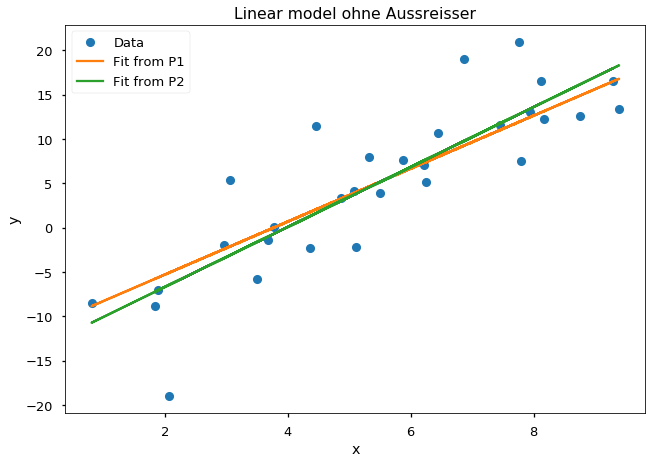
\includegraphics[width=0.8\columnwidth]{21c.png}
	\caption{\label{fig:21c} Ergebnisse der Regression ohne Ausreisser mit $(a^1, b^2) = (2.99, -11.26)$ und $(a^2, b^2) = (3.38, -13.45)$.}
\end{figure}
\par
(d) Der Code zur Lösung ist im File regression.py enthalten. Wir erkennen klar, dass das Hinzufügen von Außreissern einen stärkeren Effekt auf das Model $P_2$ hat. Dies ist wenig verwunderlich, da die quadratische Zielfunktion stärker von Außreissern beeinflusst wird. Wir sehen in Abbildung \ref{fig:21d} gut, wie die beiden Datenpunkte \glqq links-oben\grqq \ die grüne Gerade \glqq hochziehen\grqq. \par
\begin{figure}[h]
	\centering
	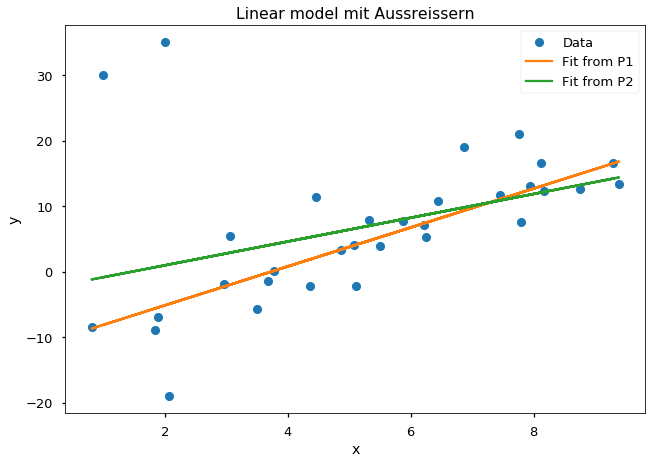
\includegraphics[width=0.8\columnwidth]{21d.png}
	\caption{\label{fig:21d} Ergebnisse der Regression mit Ausreissern mit $(a^1, b^2) = (2.97, -11.11)$ und $(a^2, b^2) = (1.82, -2.68)$.}
\end{figure}
\textbf{Aufgabe S1.3} \par
(a) Es gilt für $\bar{w}=0, \bar{b}=0, \bar{e}=1, \ (\bar{w}, \bar{b}, \bar{e}) \in M$ und damit $M\neq \emptyset$. Nun zeigen wir die Koerzivität der Zielfunktion $f: \mathbb{R}^{m+n+1} \rightarrow \mathbb{R}$, $f(w,b,e) = \frac{1}{m} \sum_{i=1}^{m}e_i + \lambda \|w \|_2^2$. Sei nun $(x^k) \subseteq M$ eine Folge mit 
\begin{equation}
	\lim\limits_{k} \| x^k \|_1 = \sum_{i=1}^{m}|e_i^k| + \sum_{i=1}^{n} |w_i^k| + |b^k|  \rightarrow \infty,
\end{equation}
dann muss also eines der Elemente der Vektoren $e$, $w$ oder $b$ betraglich gegen $\infty$ streben. Wegen $e \geq 0$ folgt weiterhin, dass $e$ nur gegen $+ \infty$ streben kann. Wegen $\| w \|_2^2 \geq 0$ folgt damit für beliebige $w$ und $b$, dass für $e_i \rightarrow \infty$ auch $\lim\limits_{k} f(w, b, e) = + \infty$ gilt. Selbiges gilt für ein beliebiges $w_i \rightarrow \pm \infty$ aufgrund der Koerzivität der Zwei-Norm. Betrachten wir nun die Fälle $b \rightarrow \pm \infty$. Wegen $\exists i,j \in \{1,...,m \} : y_i = -1, y_j = 1$ folgt, dass es mindestens ein $i$ gibt, sodass $1 - y_i (w^Tx^i + b) \infty$ für $b \rightarrow \infty$ und ein $j$ gibt sodass $1 - y_i (w^Tx^i + b) \infty$ für $b \rightarrow -\infty$. Damit folgt aus den Nebenbedingungen, dass mindestens ein Element aus $e \rightarrow \infty$ womit auch $f \rightarrow \infty$ geht. Insgesamt folgt, dass für jede Folge $(x^k) \subseteq M$ mit $\lim_k \| x^k \| \rightarrow \infty$ auch
\begin{equation*}
	\lim\limits_{k} f(x^k) = +\infty
\end{equation*}
gilt. Damit ist $f$ nach Definition 1.2.40 koerziv. Aus $M \neq \emptyset$, der Stetigkeit von $f$ (als Komposition stetiger Funktionen) und der Koerzivität von $f$ folgt mit Korollar 1.2.43 die Lösbarkeit des Problems $SVM$. \par
(b) Sei $\theta = (w^T, b, e^T)^T$, dann gilt für die Hessematrix der Zielfunktion
\begin{equation*}
	D^2 f(\theta) = \begin{pmatrix}
	2\lambda &0 &0 \\
	0 & 0 & 0 \\
	0 & 0 & 0 
	\end{pmatrix} \succeq 0
\end{equation*}
und damit, dass $f$ nach Satz 2.5.3 konvex ist. Wir merken an, dass die positive Definitiheit aus Satz 6 a) der mathematischen Grundlagen folgt, da die Eigenwerte einer Diagonalmatrix ihre Diagonalelemente sind und wegen $\lambda \geq 0$ gilt, dass der Kleinste Eigenwert der Hessematrix $0$ ist. Da die Nebenbedingungen lineare Funktionen und damit insbesondere konvexe Funktionen sind gilt mit Definition 2.1.10 und Lemma 2.1.11 das die zulässige Menge $M$ konvex ist. Aufgrund der Konvexität von $f$ und $M$ folgt mit Hilfe von Definition 2.1.15, dass es sich bei $SVM$ um ein konvexes Optimierungsproblem handelt.
\par
(c) Siehe Python. \par
(d) Siehe Python. Wir erreichen eine Accuracy von $97 \%$. Die Accuracy ergibt sich dabei als
\begin{equation}
	acc = \frac{1}{k} \sum_{i=1}^{k} \mathbf{1}_{ \{ y_i=\hat{y_i}\} }
\end{equation}
wobei $\hat{y_i} \in \{0, 1\}$ das vorhergesagte Label von Datenpunkt $i$ ist und $k$ die Anzahl an Datenpunkten in unserem Trainingsdatenset beschreibt.
\end{document}